%%
\documentclass[%
]{ittmm}


\usepackage{polyglossia}
\setdefaultlanguage[spelling=modern]{russian}
\setotherlanguages{english, german}

%%% One can fix some overfulls
\sloppy

% \usepackage{minted}
% \setminted{breaklines=true}

\addbibresource{main.bib}
\addbibresource{zotero.bib}

%% end of the preamble, start of the body of the document source.
\begin{document}

\selectlanguage{russian}

%%
%% Rights management information.
%% CC-BY is default license.
\copyrightyear{2025}
\copyrightclause{Copyright for this paper by its authors.
  Use permitted under Creative Commons License Attribution 4.0
  International (CC BY 4.0).}

%%
%% This command is for the conference information
\conference{Information and Telecommunication Technologies and Mathematical Modeling of High-Tech Systems 2025 (ITTMM 2025), Moscow, April 07--11, 2025}

%%
%% The "title" command
\title{Элементы моделирования винтового движения}
\title[mode=trans]{Elements of screw motion modeling}

% \tnotemark[1]
% \tnotetext[1]{You can use this document as the template for preparing your publication. We recommend using the latest version of the ittmm style.}

%%
%% The "author" command and its associated commands are used to define
%% the authors and their affiliations.
\author[1]{Иван А. Подмогильный}[%
trans={Ivan A. Podmogilniy},
% orcid=0,
email=1142240397@pfur.ru,
% url=https://yamadharma.github.io/,
]
\cormark[1]

\author[1]{Кирилл В. Дидусь}[%
trans={Kirill V. Didus},
% orcid=0,
email=114224340434@pfur.ru,
]

\author[1]{Мигран Н. Геворкян}[%
trans={Migran N. Gevorkyan},
% orcid=0,
email=gevorkyan-mn@rudn.ru,
]

\address[1]{Российский университет дружбы народов, ул. Миклухо-Маклая, д. 6, Москва, 117198, Российская Федерация}

%%% Footnotes
\cortext[1]{Автор, отвечающий за публикацию.}

%%
%% The abstract is a short summary of the work to be presented in the
%% article.
\begin{abstract}
  В данной работе приводится сравнительный анализ двух подходов к моделированию движения твёрдых тел. Особое внимание уделяется винтовому движению, которое является наиболее обобщённой моделью пространственного перемещения твёрдого тела. Анализ литературных источников показал, что представлено недостаточное число общедоступных примеров применения винтов в контексте геометрической визуализации, а также наглядных вычислительных примеров. Проведённое исследование направлено на восполнение пробела в прикладных методологических материалах. В работе представлено детальное описание математических формул с пояснениями. Приводятся вычислительные примеры, включая реализацию винтового движения с использованием матричного метода и формулы Родрига.
\end{abstract}

%%
%% Keywords. The author(s) should pick words that accurately describe
%% the work being presented. Separate the keywords with commas.
\begin{keywords}
  винты \sep
  моторы \sep
  вращения \sep
  трансляции \sep
  компьютерная геометрия
\end{keywords}

%% This command processes the author and affiliation and title
%% information and builds the first part of the formatted document.
\maketitle

\section{Введение}
\label{sec:intro}

При изучении литературы о математических основах компьютерной графики,
а более конкретно математического аппарата применяемого для позиционирования трехмерных объектов в
пространстве, авторы столкнулись с упоминанием таких математических объектов как моторы, винты и
бикватернионы, но без описания самого математического аппарата. Суть всех упоминаний сводилось к тому,
что этот математический аппарат позволяет вычислять вращения с одновременной трансляцией вдоль некоторой
произвольной оси, активно используется на практике, но является не интуитивным и сложным для
понимания~\cite{Lengyel:GameEngine:v1:2016} и потенциально может быть заменен геометрической алгеброй.

Поиск материалов, в которых математический аппарат моторов, винтов и бикватернионов был бы изложен во
всей полноте и последовательности, привел авторов в область физики абсолютно твердого 
тела~\cite{Chelnokov:2006}. Оказалось, что искомая теория была разработана еще на рубеже 19 и 20 веков
в основном в трудах Э.~Штуди, Р. С.~Болла~\cite[73]{KleinHoherGeometrie} и 
А. П.~Котельникова~\cite{Kotelnikov:2019}. Полноценное изложение алгебры винтов можно найти в 
монографии~\cite{Dimentberg:1965}. Более поздние работы, в том числе и на английском языке, никакого 
существенно нового материала не дают.

Найденные источники были ориентированны на теоретическую механику, поэтому все имеющиеся практические 
примеры применения винтовой и бикватернионной алгебры сводились к физике абсолютно твердого тела и к 
механике различных механизмов. Лишь один найденный источник~\cite{Goldman2024} был посвящен применению
бикватернионов к вопросам компьютерной геометрии и моделированию проективного пространства, однако полностью
обходил тему винтов и никак не упоминал крайне важный принцип перенесения Котельникова--Штуди.

Данный доклад носит методологический характер. В теоретической части авторы подробно излагают 
алгебраическую часть теории, вводят основные понятия и формулы. Во второй части приводится два расчетных
примера. Первый пример показывает винтовое движение прямой вокруг оси матричным способом 
(матрицы с дуальными коэффициентами), а второй аналогичное движение с помощью формулы Родрига.

\section{Алгебра винтов}

\subsection{Дуальные числа}
Подробно про эллиптические, параболические и гиперболические числа написано в препринте~\cite{gevorkyanApproachesImplementationGeneralized2020}.
Дуальное число $z$ определяется как:
\begin{equation*}
  z=a+\varepsilon b, \quad a,b \in \mathbb{R},\;\; \varepsilon^2=0,\;\; \varepsilon \ne 0.  
\end{equation*}

Также далее будет использоваться следующее свойство для дуальных чисел:
\begin{equation*}
  e^{\varepsilon x} = 1 + \varepsilon x
\end{equation*}

Считается что изначально дуальные числа были предложены Клиффордом~\cite{cliffordPreliminarySketchBiquaternions1871},
и в дальнейшем исследованы Штуди~\cite{zindlerGeometrieDynamenStudy1903}.

\subsection{Моторы и винты}

Мотором называется пара векторов 
\begin{equation*}
  \mathbf{R} = \{ \mathbf{v} \mid \mathbf{m} \},
\end{equation*}
где $\mathbf{v}$ - направляющий вектор прямой, $\mathbf{m}$ - момент прямой.

Мотор можно также записать в виде дуального вектора (диады): 
\begin{equation*}
  \mathbf{R} = \mathbf{v} + \varepsilon \mathbf{m}.
\end{equation*}

Для любого мотора можно подобрать такую систему координат, что в ней векторы $\mathbf{v}$ и $\mathbf{m}$ будут коллинеарны.
Винтом называется мотор, у которого направляющий вектор и момент коллинеарны $\mathbf{m} \mid \mathbf{v}$. Винт имеет запись
\begin{equation*}
  R = \{ \mathbf{v} \mid p\mathbf{v} \} = \mathbf{v} + \varepsilon p \mathbf{v} = (1+\varepsilon p)\mathbf{v}
\end{equation*}
\begin{equation*}
  p=\frac{(\mathbf{v}, \mathbf{m})}{\| \mathbf{v} \|^2},
\end{equation*}
где $p$ --- параметр винта.

Винт, у которого норма направляющего вектора равна единице $\| \mathbf{v} \| = 1$ называется единичным винтом. Любой винт можно записать через единичный:
\begin{equation*}
  R = r(1+\varepsilon p)\mathbf{E} = r e^{\varepsilon p}\mathbf{E}
\end{equation*}

Более подробно теория по винтам и моторам излагается в книге~\cite{Dimentberg:1965}.

\subsection{Принцип Штуди--Котельникова и основные формулы}

Принцип перенесения Штуди--Котельникова можно сформулировать следующим образом. Все формулы теории конечных поворотов и кинематики движения твердого тела с одной неподвижной точкой при замене в них вещественных величин на дуальные переходят, векторных величин на винтовые и кватернионов на бикватернионы, переходят в соответствующие формулы кинематики движения свободного тела (без закрепленных точек).

Матрицы элементарных поворотов Эйлера при применении принципа перенесения превращаются в матрицы винтовых движений вдоль осей $Ox$, $Oy$, $Oz$ декартовой системы координат на дуальный угол $\Theta = \theta + \theta^o \varepsilon$, где действительная часть $\theta$ задает угол поворота вокруг оси, а дуальная часть $\theta^o$ — расстояние трансляции вдоль той же оси.
\begin{equation*}
  R_x(\Theta) = 
  \begin{bmatrix}
    1 & 0 & 0\\
    0 & \cos{\Theta} & -\sin{\Theta}\\
    0 & \sin{\Theta} & \cos{\Theta}
  \end{bmatrix}
  \;\;
  R_y(\Theta) = 
  \begin{bmatrix}
    \cos\Theta & 0 & \sin\Theta\\
    0 & 1 & 0\\
    -\sin\Theta & 0 & \cos\Theta
  \end{bmatrix}
  \;\;
  R_z(\Theta) = 
  \begin{bmatrix}
    \cos\Theta & -\sin\Theta & 0\\
    \sin\Theta & \cos\Theta & 0\\
    0 & 0 & 1
  \end{bmatrix}
\end{equation*}
Функции синус и косинус от дуального угла вычисляются по следующим формулам:
\begin{equation*}
  \sin\Theta = \sin(\theta + \theta^o \varepsilon) = \sin\theta + \theta^o \cos\theta \varepsilon,\;\;
  \cos\Theta = \cos(\theta + \theta^o \varepsilon) = \cos\theta - \theta^o \sin\theta \varepsilon.
\end{equation*}

Для получения винтового аналога формулы Родрига, запишем вначале оригинальную формулу Родрига для вращения радиус вектора $\mathbf{L}$ на угол $\theta$ вокруг оси, задаваемой прямой с направляющим вектором $\mathbf{a}$, проходящей через начало координат $O$:
\begin{equation*}
  \mathbf{p}^\prime = \cos\theta \mathbf{p} + (1 - \cos\theta) (\mathbf{a}, \mathbf{p})\mathbf{a} + \sin\theta \mathbf{a}\times\mathbf{p}.
\end{equation*}
Согласно принципу перенесения, следует заменить векторы на винты, вещественные углы на дуальные. Поэтому вектор $\mathbf{p}$ должен быть заменен на винт $\mathbf{L} = \mathbf{v} + \mathbf{m} \varepsilon$, где $\mathbf{v}$ — направляющий вектор оси винта, а $\mathbf{m}$ — момент оси винта, а вектор $\mathbf{a}$ на винт $\mathbf{A} = \mathbf{a} + \mathbf{a}^o \varepsilon$, где $\mathbf{a}$ — направляющий вектор оси винта, который представляет собой ось винтового движения, а $\mathbf{a}^o$ — момент этого винта. В результате получаем формулу, которая позволяет подвергать винтовому движению винты, а не векторы:
\begin{equation*}
  \mathbf{L}^\prime = \cos\Theta \mathbf{L} + (1 - \cos\Theta) (\mathbf{A}, \mathbf{L})\mathbf{A} + \sin\Theta \mathbf{A}\times\mathbf{L}.
\end{equation*}
Так как геометрическим образом винта является прямая в пространстве, то данная формула позволяет применять винтовое движение, заданное осью $\mathbf{A}$ и дуальным углом $\Theta$, к произвольной прямой $\mathbf{L}$. Отметим, что ось $\mathbf{A}$ не привязана к началу координат и может проходить через любую точку пространства.

\section{Применение винтов для винтового движения прямой в трехмерном пространстве}

\subsection{Использование матрицы с дуальными коэффициентами}

\begin{figure}[h!]
  \centering
  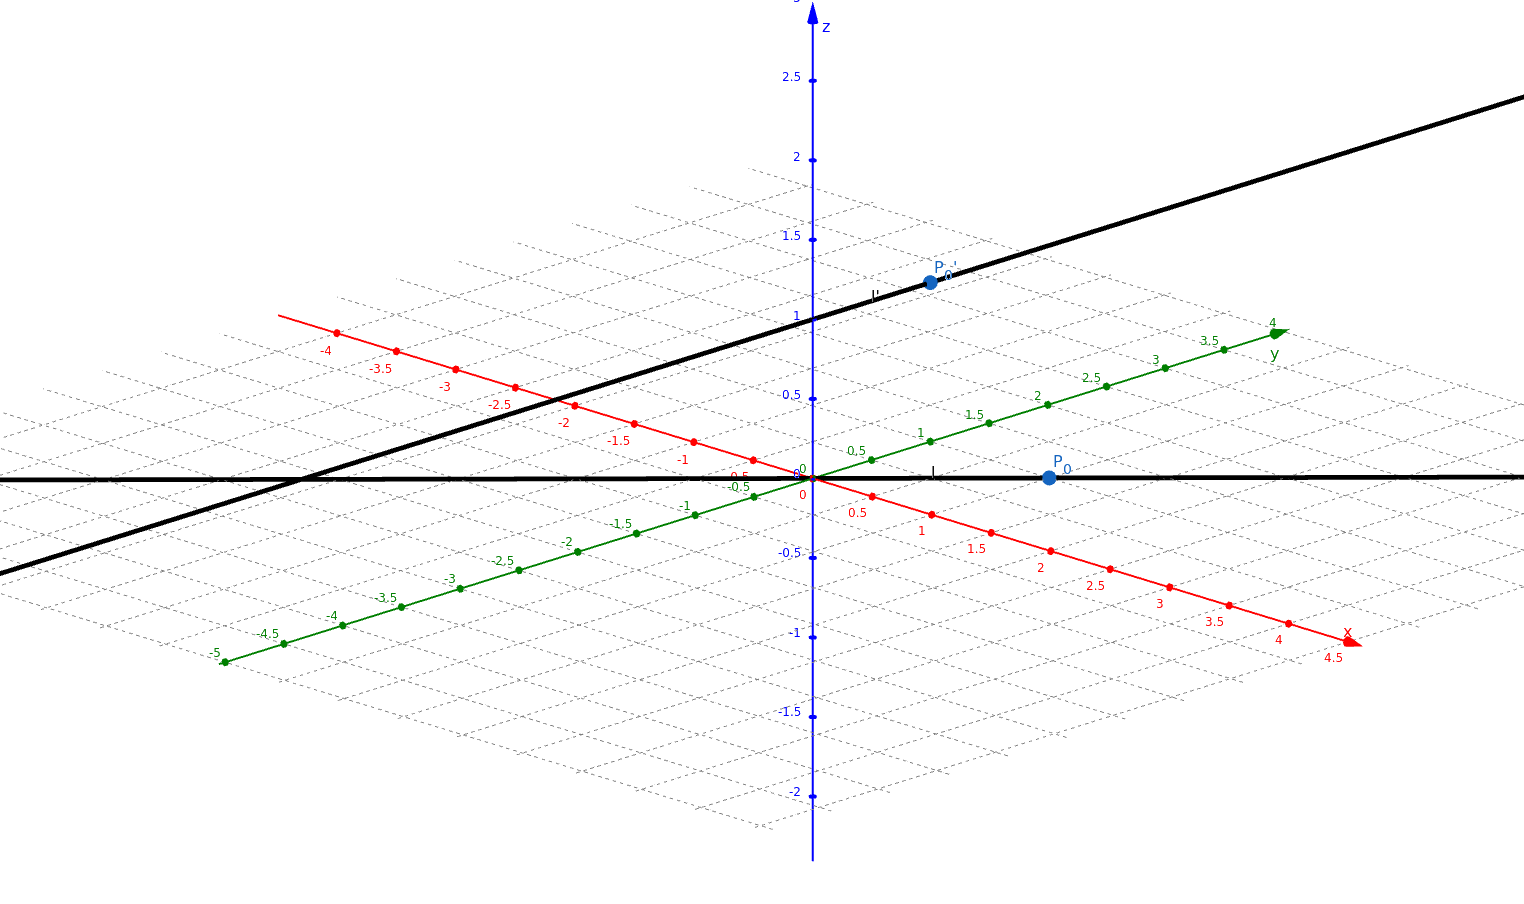
\includegraphics[width=1\textwidth]{Screw_Motion_example(1).png} % Replace with your image file
  \caption{Прямая $\mathbf{l}$ до винтового движения и прямая $\mathbf{l}'$ после винтового движения.}
  \label{fig:example}
  \end{figure}

Возьмём прямую, лежащую в плоскости $Oxy$ и проходящую через точку $O$ под углом $45^\circ$ к осям $Ox$ и $Oy$. Запишем винт, соответствующий этой прямой.
Направляющий вектор прямой $\mathbf{v}=(1,1,0)^T$. Произвольная точка прямой - точка $O=(0,0,0)^T$. Если считать, что $\mathbf{v}$ отложен от $O$, то вычислим
момент по формуле $\mathbf{m} = \mathbf{p} \times \mathbf{v}$ так как $\mathbf{p}=(0,0,0)^T$. Поэтому соответствующий прямой $l$ винт $\mathbf{l}$ можно записать как
$\mathbf{l} = (1,1,0)^T + \varepsilon (0,0,0)^T = 1 i + 1 j = \mathbf{e}_x + \mathbf{e}_y$.

Рассмотрим теперь дуальный угол $A=\alpha+\varepsilon \alpha^\circ$ взяв конкретные значения $\alpha=\pi/4$ и $\alpha^\circ=1$. С помощью этого угла повернём прямую $l$
на угол $\alpha$ против часовой стрелки вокруг оси $Oz$ и поднимем на $1$ вдоль той же оси $Oz$ (См. Рисунок \ref{fig:example}).

Чтобы это сделать запишем матрицу для вращения вокруг оси $Oz$ но заменим в ней угол на дуальный.

\begin{equation*}
  R_z(A)=
  \begin{bmatrix}
    \cos A & -\sin A & 0 \\
    \sin A & \cos A & 0 \\
    0 & 0 & 1
  \end{bmatrix}
\end{equation*}

Применим её к винту $\mathbf{l}$.

\begin{equation*}
  \mathbf{l}'=R_z(A)\mathbf{l}=
  \begin{bmatrix}
    \cos A & -\sin A & 0 \\
    \sin A & \cos A & 0 \\
    0 & 0 & 1
  \end{bmatrix}
  \begin{bmatrix}
    1 \\
    1 \\
    0
  \end{bmatrix}
  =
  \begin{bmatrix}
    \cos A - \sin A \\
    \sin A + \cos A \\
    0
  \end{bmatrix}
\end{equation*}

\begin{align*}
    \cos A - \sin A & =\cos \alpha - \varepsilon \alpha^\circ \sin \alpha - \sin \alpha - \varepsilon \alpha^\circ \cos \alpha =
  \cos \alpha - \sin \alpha - (\cos \alpha + \sin \alpha)\varepsilon \alpha^\circ \\
  \cos A + \sin A & = \cos \alpha - \varepsilon \alpha^\circ \sin \alpha + \varepsilon \alpha^\circ \cos \alpha =
  \cos \alpha + \sin \alpha + (\cos \alpha - \sin \alpha)\varepsilon \alpha^\circ
\end{align*}

Подставим $A=\pi/4+\varepsilon$ и получим

\begin{align*}
  \cos A - \sin A & = \cos \pi/4 - \sin \pi/4 + (\cos \pi/4 + \sin \pi/4)\varepsilon = \sqrt{2} \varepsilon \\
  \cos A + \sin A & = \cos \pi/4 + \sin \pi/4 + (\cos \pi/4 - \sin \pi/4)\varepsilon = \sqrt{2}
\end{align*}

Из чего следует

\begin{equation*}
  \mathbf{l}'=
  \begin{bmatrix}
    \sqrt{2} \varepsilon \\
    \sqrt{2} \\
    0
  \end{bmatrix}
  =
  \begin{bmatrix}
    0 \\
    \sqrt{2} \\
    0
  \end{bmatrix}
  + \varepsilon
  \begin{bmatrix}
    \sqrt{2} \\
    0 \\
    0
  \end{bmatrix}
\end{equation*}

Если направляющий вектор нормировать то получим:

\begin{equation*}
  \mathbf{l}' = (0,1,0)^T + \varepsilon (1,0,0)^T
\end{equation*}

% \subsection{Использование винтового аналога формулы Родрига}

\section{Заключение}
В данном тезисе был рассмотрен первый заявленный подход: винтовое движения с использованием матричного метода. 
Были кратко изложены основные формулы и определения, а также рассмотрен пример винтового движения при помощи матрицы с дуальными коэффициентами. 
В докладе планируется изложить материал по винтовому аналогу формулы Родрига и провести сравнительный анализ двух подходов. Также провести численное моделирование и опубликовать доступ к исходному коду для примеров моделирования. 


\vspace{\baselineskip}

% \begin{authorcontributions}
%   Концептуализация, написание --- рецензирование и редактирование: Анна Владиславовна Королькова; методология, написание --- подготовка первоначального варианта: Дмитрий Сергеевич Кулябов.
%   Все авторы прочитали и согласились с опубликованной версией рукописи.
% \end{authorcontributions}

\begin{funding}
  Данное исследование не получало внешнего финансирования.
\end{funding}

\begin{dataavailability}
  В ходе исследования не было создано и проанализировано никаких новых данных. Совместное использование данных неприменимо.
\end{dataavailability}

\begin{conflictsofinterest}
  Авторы заявляют об отсутствии конфликта интересов.
\end{conflictsofinterest}

\begin{acknowledgments}
  Мы благодарим организаторов конференции за предоставленную возможность создать этот тезис.
\end{acknowledgments}

%%
%% Define the bibliography file to be used
\printbibliography

\end{document}

%%% Local Variables:
%%% mode: LaTeX
%%% TeX-master: t
%%% End:
